\chapter{State of the Art}
\label{chap:sota}
\begin{spacing}{1.5}
\sloppy
In the rapidly evolving landscape of artificial intelligence (AI), large language models (LLMs) have demonstrated remarkable results in text generation and understanding. Yet, when applied to real-world tasks such as question answering, these models still face significant limitations. As detailed in the previous chapter, LLMs are prone to hallucinations\footnote{In the context of LLMs, hallucinations refer to outputs that are plausible-sounding but factually incorrect, fabricated, or unsupported by the underlying data or external sources.}, rely on static and often outdated training data, and offer limited transparency or traceability in their outputs. Additionally, they may struggle to incorporate domain-specific context or organizational knowledge \citep{vaibhav_retrieval-augmented_2025}. These factors pose challenges for domains, like cultural heritage and archaeology, where reliability, provenance, and interpretive rigor are fundamental requirements.

To address these concerns, retrieval-augmented generation (RAG)\footnote{For more information about RAG technique, see \url{https://en.wikipedia.org/wiki/Retrieval-augmented_generation}.} has emerged as a crucial methodological advance. It improves the factual grounding and contextual relevance of generated answers, thorugh the integration of external and verifiable knowledge at inference time, thereby reducing the risk of generating fabricated or distorted information \citep{martineau_what_2023}. As discussed in \autoref{chap:QAS}, this approach represents a significant step beyond both traditional information retrieval and earlier neural QA models, which were often brittle, domain-dependent, or struggled to adapt to evolving information needs.
\sloppy
The adoption of RAG in question-answering reflects a broader evolution within the field: from early symbolic and rule-based systems, through statistical and information retrieval approaches, to today’s transformer-based, generative architectures. This shift has transformed not only the technical capabilities of QA systems but also their applicability to complex, heterogeneous knowledge domains.
\sloppy
Although initially developed for open-domain question answering and enterprise search \parencite{akkiraju_facts_2024, jiang_towards_2024, packowski_optimizing_2024, yang_ragva_2025, zhou_enabling_2025}, RAG pipelines are increasingly adopted in the humanities and cultural heritage contexts. In these sectors, where interpretive rigor, provenance, and information reliability are critical, RAG-based tools support scholars and professionals in navigating vast, fragmented knowledge repositories. While some initiatives employ RAG to analyze sensitive historical materials \citep{callaghan_prototyping_2025, ciletti_retrieval-augmented_2025, sergeev_talking_2025, fan_research_2025}, this thesis explores a distinct application: improving access to procedural and technical documentation, where clarity, consistency, and actionable guidance are the primary objectives.
\\

This chapter therefore provides a comprehensive overview of the state of the art in retrieval-augmented generation, situates RAG within the current research landscape, outlines its core mechanisms, and examines its recent application in the digital humanities.

\section{Core Mechanisms and Foundations of Retrieval-Augmented Generation}\setlength{\parskip}
{0pt}
Retrieval-augmented generation (RAG) is a hybrid approach that addresses key limitations of traditional LLMs, knowledge staleness, limited context awareness, and lack of output traceability \parencite{vaibhav_retrieval-augmented_2025,gao_retrieval-augmented_2024, gupta_comprehensive_2024}. While LLMs excel in generating fluent, human-like text, they often falter when facing domain-specific queries or requests for information beyond their training cutoff. RAG directly addresses these challenges by integrating external information retrieval within the generation process, ensuring outputs are more factual, current, and grounded in verifiable sources \citep{wang_searching_2024}.

The RAG pipeline typically consists of two main stages: \textbf{retrieval} and \textbf{generation} (\cite{odsc-community_retrieval-augmented_2024}). The process begins with indexing, where raw data is cleaned, extracted, segmented into manageable "chunks", and encoded into vector representations. These embeddings are then stored in a vector database to facilitate efficient similarity searches. Upon receiving a user query, the system encodes it into a vector and retrieves the top-k most relevant chunks from the indexed knowledge base. In the second stage, the retrieved documents are passed to a generative model, often built upon Transformer architectures \citep{vaswani_attention_2017}. This module synthesizes the original query with the retrieved information to formulate a well-informed, coherent, and contextually appropriate response \citep{arslan_survey_2024}.

This modular mechanism (\autoref{fig:rag}) overcomes the limitations of static model parameters by continuously incorporating domain-specific and updated information. Recent contributions have helped to formally systematize the RAG pipeline's, with frameworks delineating specific interdependent modules such as query classification, retrieval, re-ranking, and generation \parencite{wang_searching_2024}.

\vspace{0.5em}
\begin{figure}[H]
  \centering
  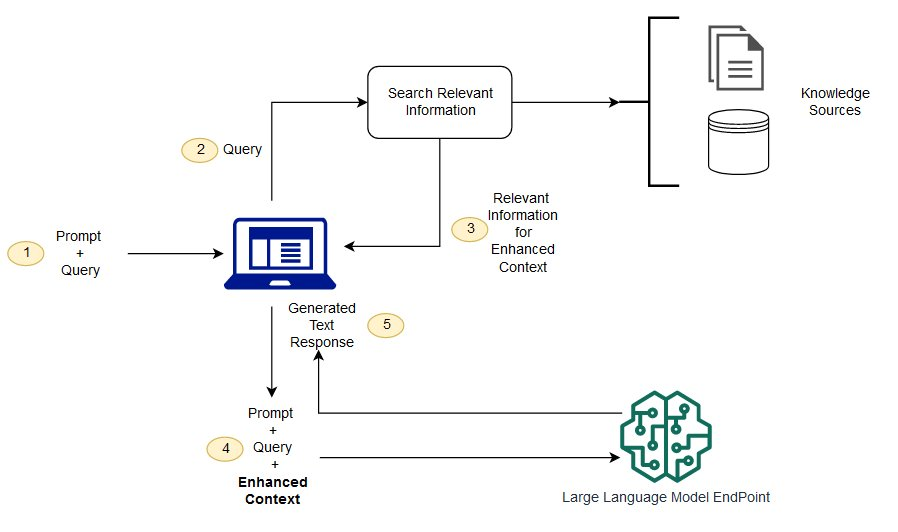
\includegraphics[width=\textwidth]{images/rag_workflow.jpg} 
  \caption{Typical RAG workflow.\\
  \footnotesize{Source: \url{https://aws.amazon.com/de/what-is/retrieval-augmented-generation/}.\nocite{noauthor_was_nodate}}}
  \label{fig:rag}
\end{figure}
\vspace{0.5em}

\noindent In summary, the synergistic merging of LLMs' intrinsic knowledge with dynamic external sources allows for continuous knowledge updates and integration of domain-specific information, significantly enhancing response quality, particularly in knowledge-intensive and evolving domains \parencite{wang_searching_2024, gao_retrieval-augmented_2024}.

\section{Emerging Applications and Use Cases}\label{sec:evol_qas}
RAG systems are increasingly deployed across diverse domains -- spanning academia, enterprise, and product environments -- to enhance data accessibility, support decision-making, and facilitate natural language interaction with complex knowledge bases. Recent surveys and empirical studies document a growing array of scholarly applications of RAG, including:
\begin{itemize}
    \item Automated literature review tools and citation management -- e.g., LitLLM; \citep{agarwal_litllm_2025}, KNIMEZoBot; \citep{alshammari_knimezobot_2023};
    \item Generation of summaries for large corpora of academic papers;
    \item Field-specific knowledge extraction, including biomedical and legal research support.
\end{itemize}

\noindent In one experiment, a RAG system was developed to assist data scientists through a combination of GROBID for structured bibliographic extraction, fine-tuned embeddings, semantic chunking, and an abstract-first retrieval strategy. The system's performance, assessed using the Retrieval-augmented generation Assessment System (RAGAS), demonstrated improved faithfulness and context relevance in response generation \citep{aytar_retrieval-augmented_2024}. A similar approach was explored in the context of academic library systems, where RAG was applied to improve contextual retrieval through semantic indexing of structured metadata (e.g., MARC/RDA standards) and multimodal resources. Additionally, the framework introduced conversational querying via a natural language interface, supporting complex interdisciplinary searches and significantly improving document discoverability by synthesizing citation-backed responses from diverse scholarly sources -- including journals, datasets, and videos. This solution also addressed challenges such as copyright compliance and ethical AI transparency \citep{bevara_prospects_2025}.  Collectively, these studies affirm RAG systems’ efficacy in alleviating information overload and improving research workflow discoverability.

In parallel, the work of \citep{soman_observations_2024} provides further critical insights into the design of RAG systems for domain-specific and technical content, closely aligning with the methodological framework adopted in the GNA question-answering system. Using IEEE telecommunications engineering corpora (i.e., wireless LAN specifications and battery glossaries) as testbeds, their analysis highlights key factors influencing retrieval quality, which include chunk size, sentence-level similarity, and the strategic placement of domain-specific terms. These aspects are similarly addressed in the GNA RAG pipeline \citep{pograri_question-answering_2025}, which applies customized tailored chunking, semantic preprocessing, and contextual embedding strategies. Both studies advocate for more nuanced, context-aware approaches to enhance precision in technical and highly structured domains.

Numerous recent graduate-level research projects have provided substantive input into the implementation and evaluation of RAG systems:
\begin{itemize}
    \item \textcite{antolini_experimental_2025} developed a custom RAG system for open-domain question answering using both traditional (BM25, PRF) and advanced retrieval strategies, integrated with local LLMs. A novel Parametric RAG (PRAG) approach was also explored, embedding context into model parameters for performance gains.
    \item \textcite{caramanna_progettazione_2024} investigated conversational agent architectures, comparing various LLM types and retrieval configurations.
    \item \textcite{florio_progettazione_2024} implemented a LangChain-based RAG chatbot for corporate documentation, evaluating multiple vector database technologies.
    \item \textcite{salcuni_utilizzo_2025} applied RAG to the medical domain, improving LLM responses in hypertension care. The study used RAGAS to assess quality and relevance, focusing on personalization and accuracy.
    \item \textcite{nicoletti_llms_2025} developed Essence Coach, a chatbot that integrates LLMs with the Essence software engineering standard. This system significantly outperformed generic LLMs like GPT-4o in domain-specific reasoning tasks.
\end{itemize}

\section{RAG in the Digital Humanities}
A growing body of research is exploring RAG applications within the digital humanities. One such example is the \textit{iREAL} project, which applied RAG to interpret archival records from Aboriginal schools in Australia, demonstrating a careful balance between cultural sensitivity and historical accuracy \citep{callaghan_prototyping_2025}. Another initiative, \textit{ValuesRAG}, focuses on cultural alignment in LLMs by integrating societal and demographic knowledge through retrieval-augmented contextual learning, experimenting with the \textit{World Values Survey} dataset \citep{seo_valuesrag_2025}. In another case, the \textit{Foggia Occupator Dataset} project applied a RAG model to post-WWII Italian periodicals, extracting information on political figures and stylistic traits \citep{ciletti_retrieval-augmented_2025}.

RAG methodologies are being adopted within the GLAM sector (Galleries, Libraries, Archives and Museums) as well. In archival contexts, a smart assistant developed for querying the \textit{Prozhito} digital archive of personal diaries combines text-to-SQL filtering, hybrid search, and automatic query reformulation, proving especially effective for historians and anthropologists without prior knowledge of database query languages  \citep{sergeev_talking_2025}. Meanwhile, in museum settings, a comparative evaluation of RAG systems versus large-context LLMs for answering multimodal questions about artworks demonstrated that the RAG approach offers superior precision and explainability \citep{ramos-varela_context_2025}.

Innovations in graph-based retrieval are also gaining momentum \citep{belagatti_enhance_2024}. Techniques combining structured supervision and chain-of-thought prompting have been used to map character relationships in early modern English historiography, thereby reducing the manual workload typically associated with historical data annotation \citep{fan_research_2025}. Related directions are being explored within cultural heritage institutions, as seen in the \textit{CAT-IA} initiative \citep{barbato_nasce_2025}, which integrates ArCo knowledge graph \citep{carriero_arco_2019} within a RAG system for provenance tracking, AI explainability (XAI), and structured metadata extraction. Designed to streamline and enrich user interactions with the General Catalogue of Cultural Heritage \textit{(Catalogo generale dei beni culturali)}, \textit{CAT-IA} marks a notable stride in applying advanced digital technologies to promote accessibility and valorization of cultural assets.

Finally, efforts to advance access to fragmented digital repositories -- such as web archives -- have increasingly adopted RAG methodologies. An illustrative bespoke prototype \citep{davis_unlocking_2025} transforms keyword-based search into semantically guided question answering, sharing architectural parallels with the GNA QA system presented in the context of this thesis. Both systems prioritize semantic retrieval over lexical matching using dense embeddings -- e.g., \textit{E5} variants \citep{wang_text_2024} -- to interpret queries in context, employ structured text processing pipelines to reduce noise in source materials, and apply optimized chunking strategies for retrieval accuracy. Crucially, these studies highlight RAG’s potential to transform scattered and heterogeneous resources -- whether web archives or catalographic procedures -- into coherent, accessible knowledge through context-aware synthesis.

\section{Future Directions}
Ongoing research is pushing the boundaries of RAG, exploring innovative directions such as synthetic corpus generation, autonomous agent behavior, and AI-driven creative processes. One promising approach involves using synthetic corpora to enhance the robustness of RAG systems, improving their ability to generalize in low-resource domains \citep{bor-woei_generative_2024}. RAG is also increasingly applied to automate literature reviews and research synthesis. Agentic AI, such as the \textit{PaperQA} system \citep{lala_paperqa_2023}, has demonstrated the capacity to systematically retrieve and summarize academic literature through recursive querying and decision-making agents, enabling rigorous yet scalable analysis that holds significant potential for humanities scholarship \citep{han_automating_2024}.

\subsubsection*{Generative AI and Large‑Scale Agentic QA}
Large Language Models (LLMs) and prompting
After GPT‑1 (2018) and GPT‑2/3, large-scale decoder‑only models shifted capabilities: GPT‑3 in 2020 introduced few‑shot prompting and instruction‑based QA without fine-tuning.

These systems often serve as QA agents—able to plan, retrieve, reason, and generate in one pipeline, especially in retrieval‑augmented generation (RAG) frameworks.

QA as an agentic pipeline
Recent architectures treat QA as multi-stage agents: question understanding, retrieval (possibly over the web or knowledge stores), planning, reasoning, and generative answer synthesis. These yield state-of-the-art results beyond extractive systems.
(Yue 2025)
---------------------

Another significant advancement lies in semantic alignment. The integration of ontologies and knowledge graphs into RAG systems has rapidly advanced both the capabilities and the trustworthiness of LLMs. Ontologies, as formal domain knowledge models, provide structured frameworks that enable precise retrieval, semantic coherence, and the inclusion of ethical dimensions in generative AI. Complementing this, knowledge graphs capture complex relationships and support context-aware multi-hop reasoning, improving accuracy, explainability, and cultural sensitivity of outputs. Current research and practical applications span a range of initiatives – from ontology-guided entity typing to the grounding of AI in ethical principles and industrial procedure knowledge, demonstrating that these semantic tools are essential for creating robust, context-aware, and transparent RAG systems, addressing challenges in fields as diverse as healthcare, engineering, scientific discovery, and enterprise knowledge management \citep{tiwari_ontorag_2025, ludwig_ontology-based_2025, bran_ontology-retrieval_2024, sharma_og-rag_2024, xiao_orag_2024, park_ontology-based_2024, debellis_integrating_2024} + franco et al. 2020.

These advancements highlight the critical importance of developing RAG systems that complement rather than replace human interpretive judgment. Emerging approaches such as graph-RAG, ontology-aware models, multimodal architectures, and hybrid retrieval mechanisms represent key technical directions that support humanistic inquiry while upholding the epistemic and ethical standards of the field. Ultimately, RAG not only offers improved access to information, but also invites a reimagining of the relationship between artificial intelligence and cultural knowledge production, fostering tools that augment – not displace – human creativity and understanding.
\end{spacing}